%% ----------------------------------------------------------------------------
% BIWI SA/MA thesis template
%
% Created 09/29/2006 by Andreas Ess
% Extended 13/02/2009 by Jan Lesniak - jlesniak@vision.ee.ethz.ch
%% ----------------------------------------------------------------------------
\newpage
\chapter{Materials and Methods}
The objectives of the ``Materials and Methods'' section are the following:
\begin{itemize}
    \item \textit{What are tools and methods you used?} Introduce the environment, in which your work has taken place - this can be a software package, a device or a system description. Make sure sufficiently detailed descriptions of the algorithms and concepts (e.g. math) you used shall be placed here.
    \item \textit{What is your work?} Describe (perhaps in a separate chapter) the key component of your work, e.g. an algorithm or software framework you have developed.
\end{itemize}


\chapter{Generative Machine Learning}
\section{Bayesian Formulation of Latent Variable Models}
Before getting started it is important to define the terms used in the next sections, since they all stem from Bayesian
statistics. The Bayesian theorem can be written as
\begin{equation}
    p(z|x) = \frac{p(x|z)p(z)}{p(x)}
\end{equation}
where it is implicitly assumed that $p$ is a probability density function over two continuous random variables $x$ and $z$. The formula holds in general, but in generative modeling and machine learning it is usually assumed that the letter $z$ represents a random variable in latent space (unobserved) from which -- after training -- can be sampled to generate new data, whereas $x$ is the random variable that represents the training samples (observed space).

Using above described ordering, the four terms in this formula use distinct names:
\begin{description}
    \item[$p(x)$] is called the \textit{evidence} or the \textit{marginal likelihood}. It encompasses the actual observations of the data.
    \item[] \item[$p(z)$] is called the \textit{prior}, since it exposes information on $z$ before any conditioning.
    \item[$p(z|x)$] is called the \textit{posterior}. It describes the distribution over $z$ after (\textit{post}) having seen the evidence $x$.
    \item[$p(x|z)$] is called the \textit{likelihood}. It gives the literal likelihood of observing an example $x$ when choosing the latent space to be a specific $z$.
\end{description}

\section{Variational Autoencoders}
One of the most straightforward examples of a generative model, where the goal is to find such a latent space representation of the training sample distribution, is the Variational Autoencoder (VAE)~\autocite{kingma2022autoencoding}. The name of the VAE stems from the Autoencoder, a network that tries to recreate its output through a bottleneck and thereby learns a compressed representation of the data.~\autocite{https://doi.org/10.1002/aic.690370209} Autoencoders bear similarity to other dimension reduction methods like Principal Component Analysis (PCA) and therefore were first published under the name \textit{Nonlinear principal component analysis}. The \textit{variational} part in the VAE stems from the fact that it does not learn to recreate input samples, but is rather optimized to represent the distribution over the training samples as a combination of a parameterized latent distribution $p_{\theta_z}(z)$ and a neural network mapping $p_{\theta_{NN}}(x|z)$ between the latent space and the sample space. The latent distribution is chosen such that sampling from it is easy, which allows the neural network to create new data samples (e.g. a multivariate Gaussian).

Marginalizing $p_\theta(x) = \int p_{\theta_{NN}}(x|z) p_{\theta_z}(z) dz = \frac{p_{\theta_{NN_{out}}}(x|z) p_{\theta_z}(z)}{p_{\theta_{NN_{in}}}(z|x)}$ requires another approximation of the intractable posterior $p_{\theta_{NN_{in}}}(z|x)$ during training. A schematic of a VAE is shown in Fig.~\ref{fig:vae}.

The neural networks usually do not contain stochastic layers, but are deterministic mappings between latent space and sample space $x \sim p_{\theta_{NN_{out}}}(x|z) \Rightarrow x = f_{\theta_{NN_{out}}}(z)$. The hope is, that after training the encoder $p_{\theta_{NN_{in}}}$ can be removed and sampling from $z$ is the same as sampling from $x$.

\begin{figure}[h]
    \centering
    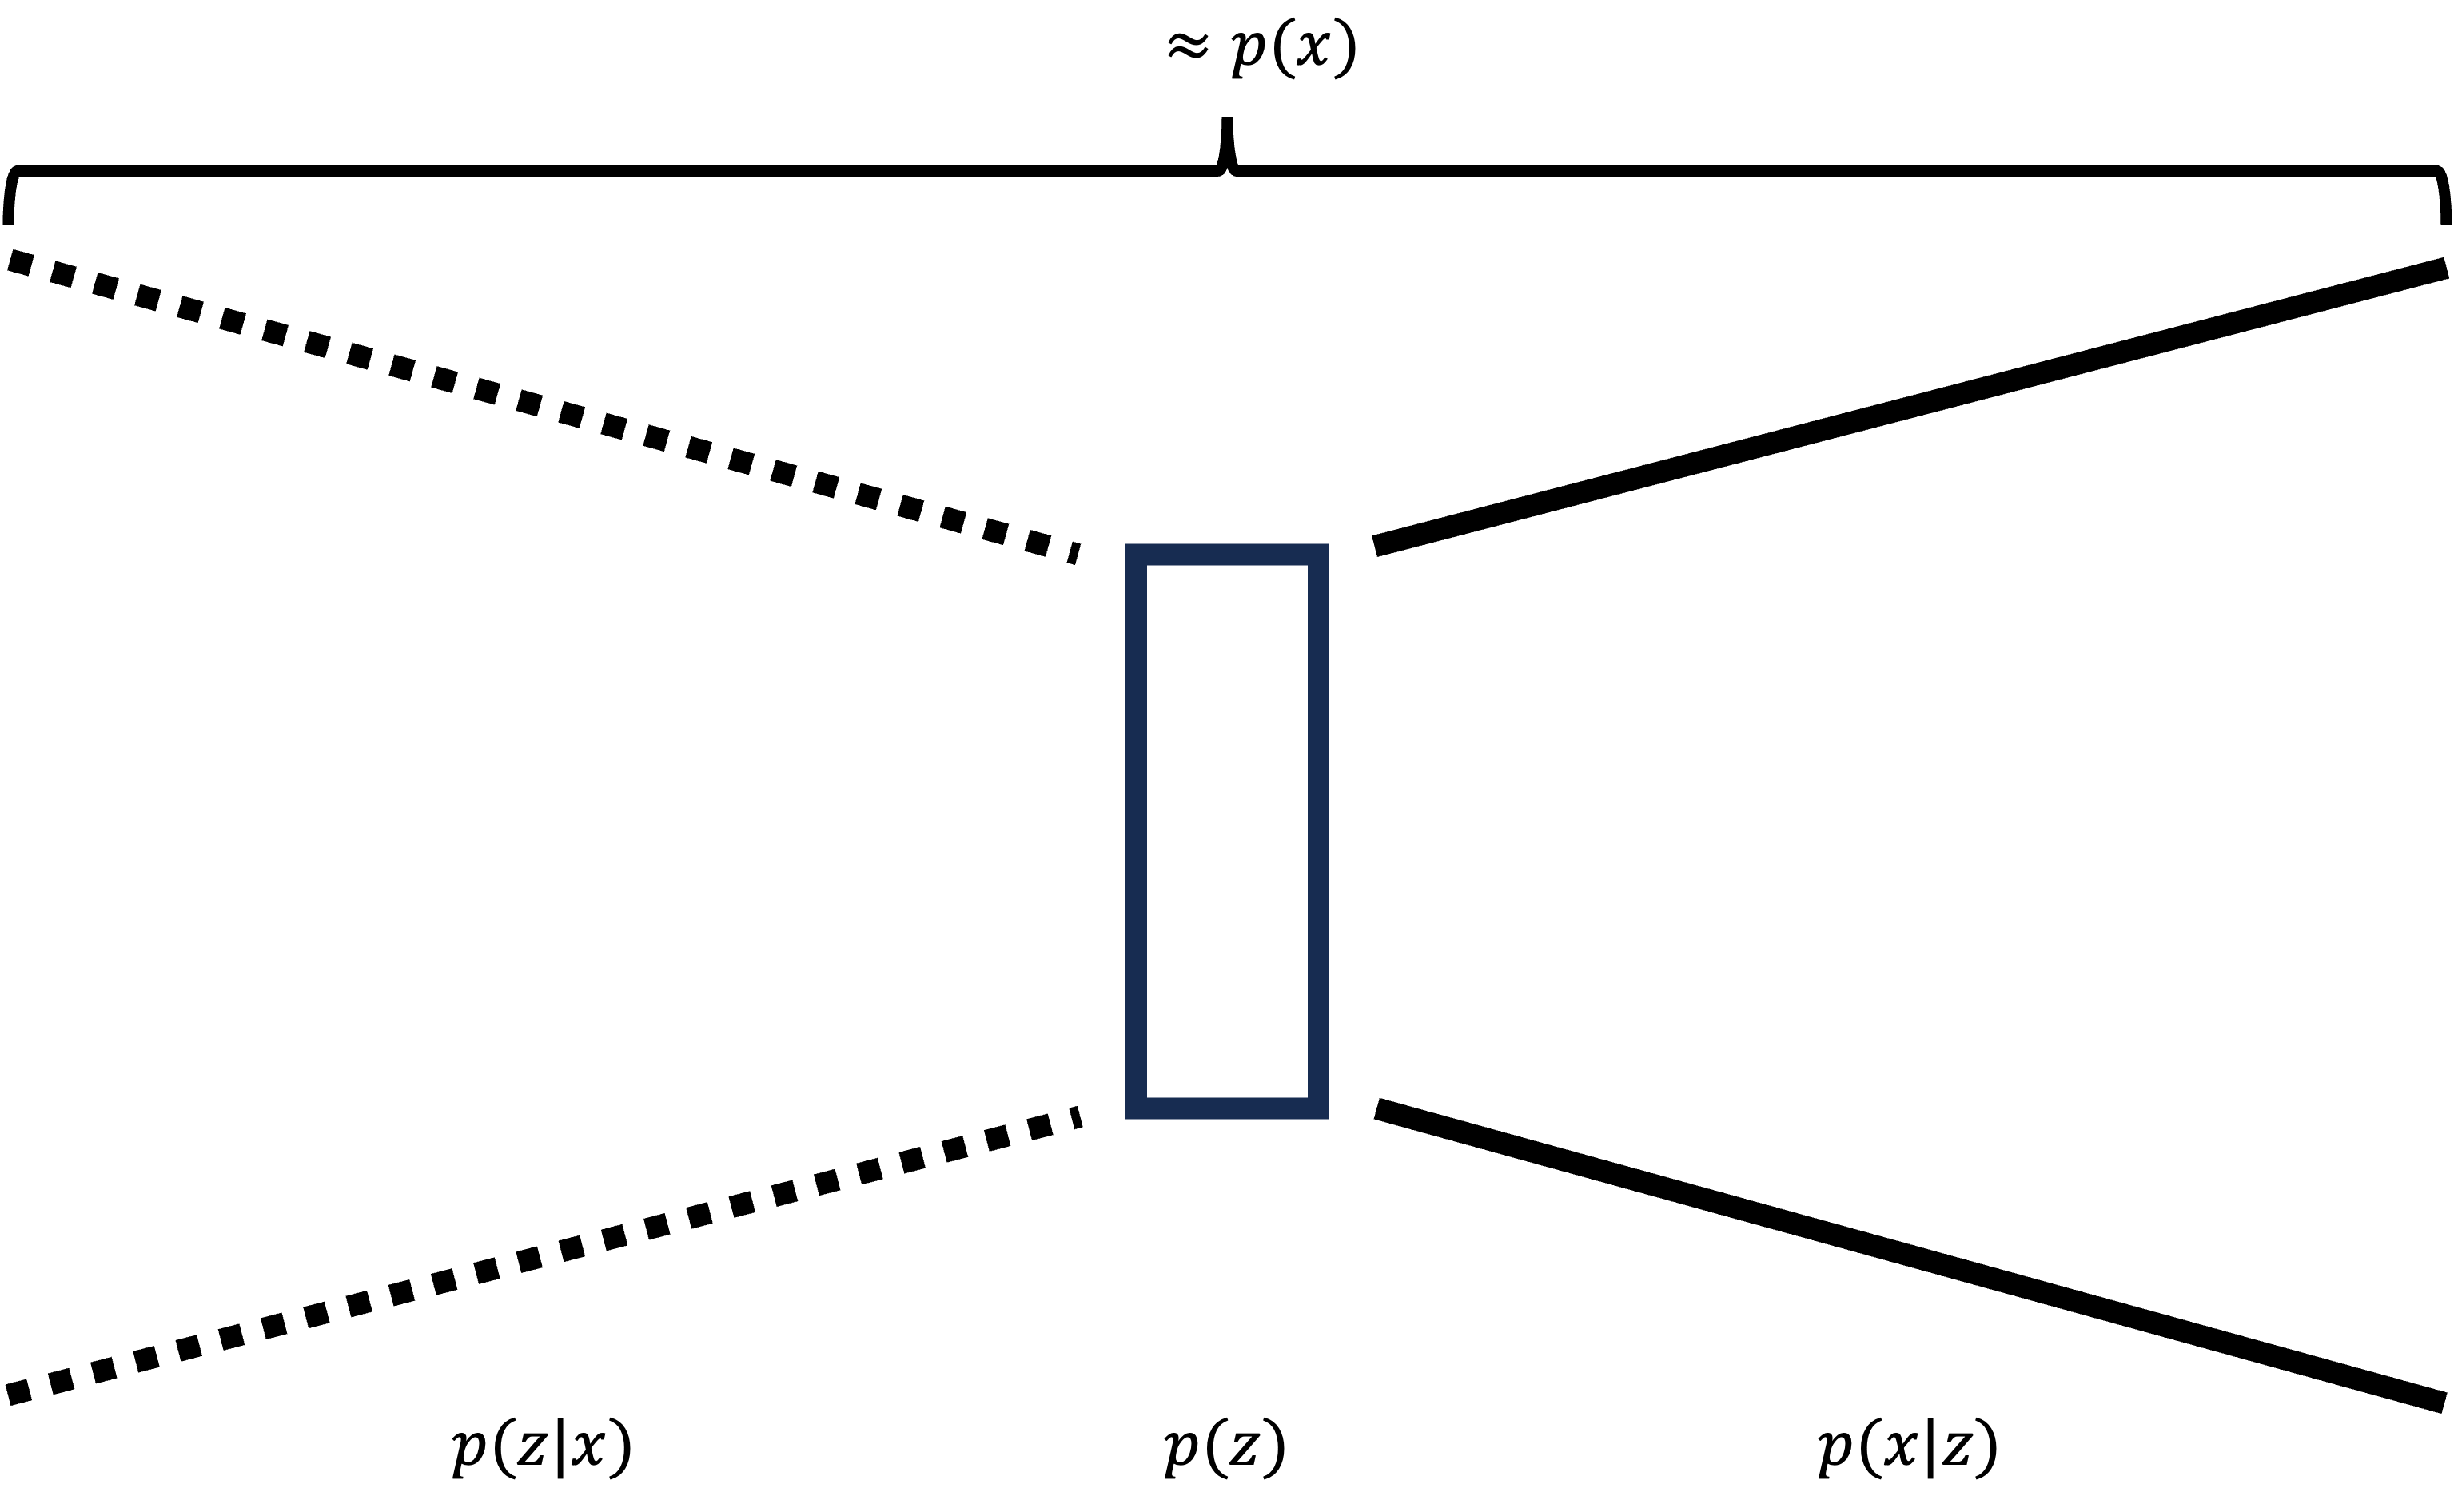
\includegraphics[width=.5\textwidth]{images/vae.png}
    \caption{VAE schematic: $p(x)$ is approximated through a latent variable model where posterior and likelihood are modeled with neural networks and the prior on the latent variable is modeled through a simple parameterized distribution (often Gaussian). The hope is, that after training, sampling from $p(z)$ and passing it through the neural network $p_{\theta_{NN}}(x|z)$, is the same as sampling from $p(x)$.}
    \label{fig:vae}
\end{figure}

\section{Diffusion Denoising Probabilistic Models}
Diffusion Denoising Probabilistic Models (DDPMs or Diffusion Models) are a generative model that learn the distribution of images in a training set. During training, sample images are gradually destroyed by adding noise over many iterations and a neural network is trained, such that these steps can be inverted.

As the name suggests, image content is diffused in timesteps, therefore we use the random variable $\bm{x}_0$ to represent our original training images, $\bm{x}_t$ for (partially noisy) images at an intermediate timestep and $\bm{x}_T$ for images at the end of the process where almost all information has been destroyed and the distribution $q(\bm{x}_T)$ largely follows an isotropic Gaussian distribution -- a Gaussian distribution with the identity matrix as covariance matrix, but a non-zero means vector.

Once the network is trained to create a less noisy image $\bm{x}_{t-1}$ from $\bm{x}_t$, we should be able to sample some new $\bm{x}_T$ and generate new samples from the training distribution $q(\bm{x}_0)$ by passing it many times through the network until all noise is removed.

\subsection{Forward Diffusion Process}
\subsubsection{Mathematical Description}
In order to derive a training objective it is important to understand the workings of the \textit{forward diffusion process}. During this process, i.i.d (independent and identically distributed) Gaussian noise is applied to the image over many discrete timesteps. A \textit{variance schedule} defines the means at variances ($\sqrt{1-\beta}$ and $\beta$) of the added noise at every timestep.~\autocite{ho2020denoising} The whole process can be expressed as a Markov chain (depicted in Fig.~\ref{fig:forward_diffusion})
\begin{equation}
    q(\bm{x}_T|\bm{x}_0) = q(\bm{x}_0) \prod_{t=1}^{T} q(\bm{x}_{t}|\bm{x}_{t-1})
\end{equation}
with the transition distributions $q(\bm{x}_t|\bm{x}_{t-1}) = \mathcal{N}(\sqrt{1-\beta_t} \bm{x}_{t-1}, \beta_t I)$. An example of iterative destruction of an image by this process is shown in Fig.~\ref{fig:forward_naoshima}.

\begin{figure}[h]
    \centering
    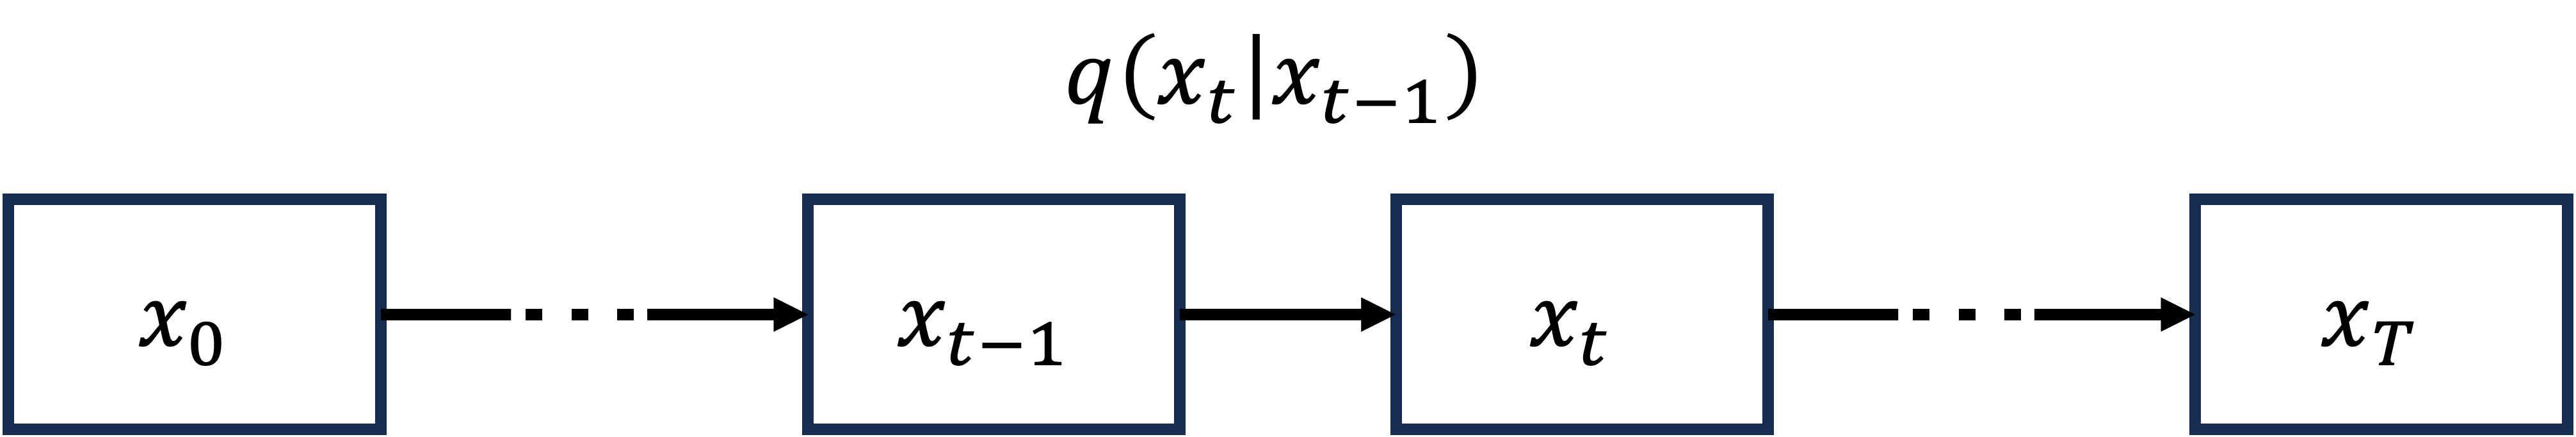
\includegraphics[width=.5\textwidth]{images/forward_diffusion.png}
    \caption{Forward Diffusion Process: An image is iteratively destroyed by adding normally distributed noise,
        according to a schedule. This represents a Markov process with the transition probability $q(\bm{x}_t|\bm{x}_{t-1})$.}
    \label{fig:forward_diffusion}
\end{figure}

\begin{figure}[h]
    \centering
    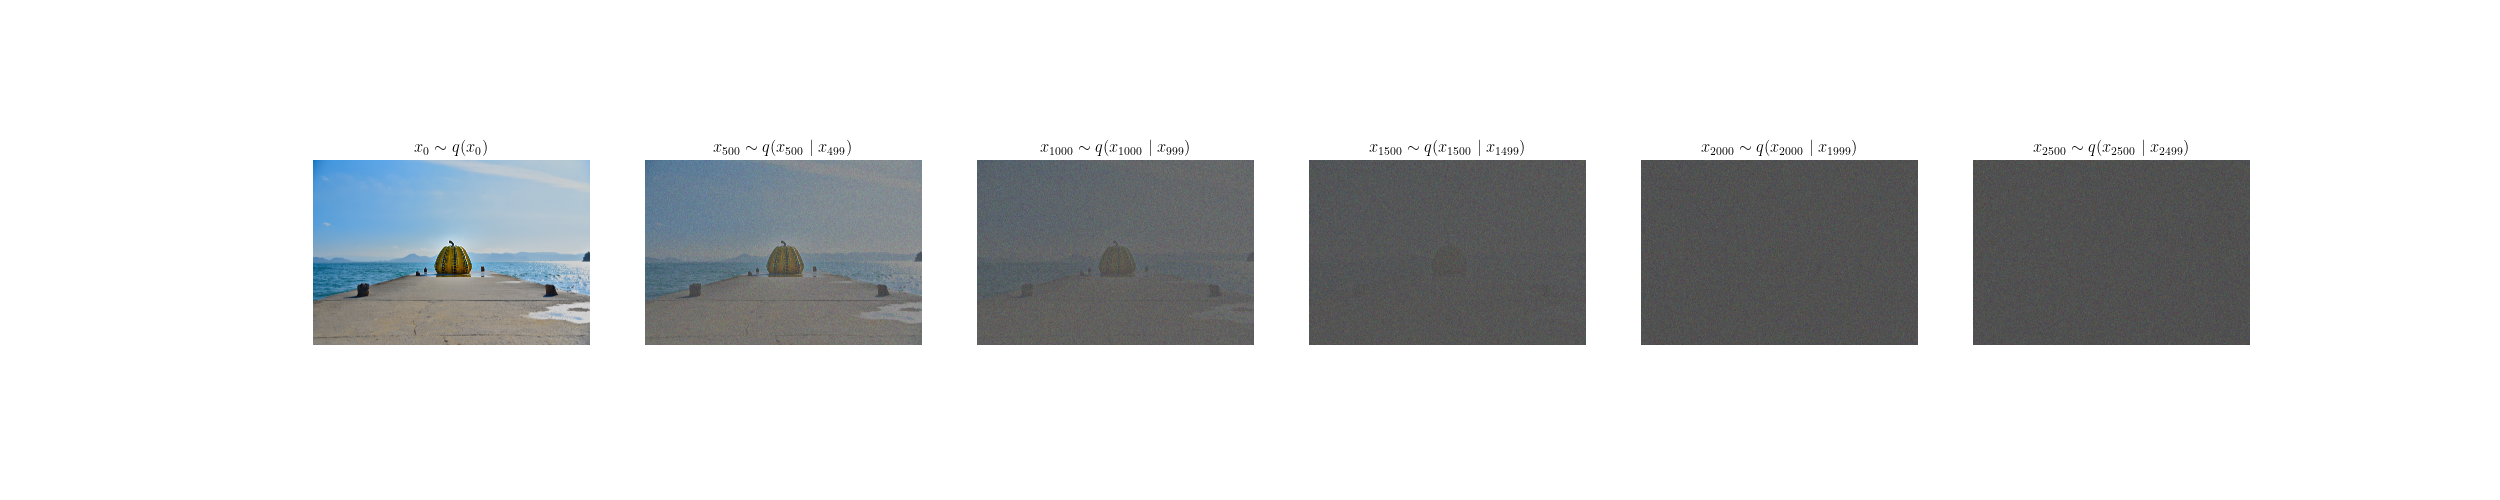
\includegraphics[width=\textwidth]{images/forward_naoshima.png}
    \caption{Example of Iterative Image Destruction through Forward Diffusion Process:
        The indices give the time step in the iterative destruction process, where $\beta$ was created according to a linear noise variance schedule (5000 steps from in the 0.001 to 0.02 range and picture resolution of 4016 by 6016 pixels).}
    \label{fig:forward_naoshima}
\end{figure}

Gladly it is not necessary to sample noise again and again in order to arrive at $\bm{x}_t$, since Ho et al. derived a closed-form solution to the sampling procedure.~\autocite{ho2020denoising} For this, the variance schedule is first reparameterized as $1-\beta = \alpha$
\begin{equation}
    q(\bm{x}_t | \bm{x}_{t-1}) = \mathcal{N}(\sqrt{\alpha_t} \bm{x}_{t-1}, (1-\alpha_t) \bm{I})
    \label{eq:forward_alpha}
\end{equation}
and the closed-form solution for $q(\bm{x}_t|\bm{x}_0)$ is derived by introducing the cumulative product $\bar{\alpha_t} = \prod_{s=1}^{t}\alpha_s$ as
\begin{equation}
    q(\bm{x}_t|\bm{x}_0) = \mathcal{N}(\sqrt{\bar{\alpha_t}}\bm{x}_0, (1-\bar{\alpha_t})\bm{I})
    \label{eq:forward_alphadash}
\end{equation}
The derivation that leads from Eq.~\ref{eq:forward_alpha} to Eq.~\ref{eq:forward_alphadash} will be left to appendix~\ref{app:forward}.

\subsubsection{Influence of Scheduling Functions}
The process of information destruction is dependent on the chosen variance schedule, the number of steps and the image size. Beyond the most simple case -- a constant variance over time -- Ho et al. opted for the second most simple option, a linear schedule, where the variance $\beta_t$ grows linearly in $t$.~\autocite{ho2020denoising} Nichol et al. later found that a cosine-based schedule gives better results, since it does not destruct information quite as quickly, making it more informative in the last few timesteps.~\autocite{nichol2021improved} Own experiments exploring above mentioned parameters are explained in~\ref{sec:forward_diff_experiments}.

\subsection{Reverse Diffusion Process}
DDPMs can be viewed as latent space models in a similar way that Generative Adversarial Nets or Variational Autoencoders can.~\autocite{goodfellow2014generative,kingma2022autoencoding}

In DDPMs the reverse process is again a Markov chain and can therefore again be factorized
\begin{equation}
    q(\bm{x}_0|\bm{x}_T) = q(\bm{x}_T) \prod_{t=T}^{1} q(\bm{x}_{t-1}|\bm{x}_{t})
\end{equation}
which means that our network does not learn to approximate the full inversion, but rather just the transition probabilities $q(\bm{x}_{t-1}|\bm{x}_{t})$ in the chain, which are transitions between several intermediate latent distributions.

\section{Latent Variable Models Compared}
\begin{table}[h]
    \centering
    \begin{tabular}{l | p{40mm} | p{40mm} | p{40mm}}
                   & VAE                                             & GAN                                             & DDPM                                                                                                                                           \\
        \hline\hline
        prior      & $p(z)$, parameterized of any shape              & $p(z)$, parameterized of any shape              & $p(\bm{x}_t)$, same shape as samples                                                                                                           \\
        posterior  & $p(z|x)$, modeled with neural network           & $p(z|x)$, modeled with loss function            & $q(\bm{x}_t|\bm{x}_{t-1})$, modeled as step in forward diffusion process                                                                       \\
        likelihood & $p(x|z)=f_{NN}(z)$, modeled with neural network & $p(x|z)=f_{NN}(z)$, modeled with neural network & $q(\bm{x}_{t-1}|\bm{x}_{t}) = \mathcal{N}(k_1 f_{NN}, k_2 f_{NN})$, modeled with Gaussian sampling with parameters estimated by neural network
    \end{tabular}
\end{table}

\section{Loss Functions}
In generative machine learning we would want our model to learn the distribution that generated
out training examples. Often this distribution is conditioned on some description (e.g. text) or
on the corruption process in our case, where we use generative models to solve inverse problems.
Assuming our original data distribution (of images) is $p(x)$, then we try to find a parameterized
variational machine learning model ($q_{\theta}(x)$) that will closely match the data distribution.

In order for this $q_{\theta}(x)$ to be trained we need a differentiable loss function that expresses
\enquote{closeness} in a distributional sense. The usual approach to this is to use the Kullback-Leibler (KL)
divergence.

\subsection{Kullback-Leibler Divergence}

\subsection{Wasserstein Distance}
A different approach to comparing the similarity of distributions is the Wasserstein metric, successfully used in the Wasserstein GAN.~\autocite{arjovsky2017wasserstein}.

\subsection{Variational Lower Bound}
As mentioned previously, the goal is to approximate a true data distribution $p^*(x)$ with a parameterized distribution $p_\theta(x) = \int p_\theta(x|z)p(z)dz$, from which sampling is easy, since the prior $p(z)$ is very simple.